\documentclass[a4paper, czech]{article}

\usepackage[czech]{babel}
\usepackage{indentfirst}
\usepackage{graphicx}
\usepackage{float}
\usepackage[margin=1.5cm]{geometry}
\usepackage{booktabs}
\usepackage{amsmath}
\usepackage{xcolor}
\usepackage{multirow}
\usepackage{tabularray}
\usepackage{bold-extra}

\begin{document}
\begin{table}[H]
    \centering
    \begin{tblr}{
        cell{1}{1} = {c = 2, r = 4}{c}, % Logo
        cell{1}{4} = {c = 3}{c}, % Předmět
        cell{2}{4} = {c = 3}{c}, % Jméno
        cell{3}{4} = {}{c}, % Ročník
        cell{3}{6} = {}{c}, % Studijní skupina
        cell{4}{4} = {}{c}, % Spolupracoval
        cell{4}{6} = {}{c}, % Mereno dne
        cell{5}{1} = {c = 2}{55mm}, % Kontroloval
        cell{5}{3} = {c = 2}{55mm}, % Hodnoceni
        cell{5}{5} = {c = 2}{55mm}, % Dne
        cell{6}{2} = {c = 5}{}, % Nazev ulohy
        cell{7}{1} = {}{c}, % Číslo úlohy
        cell{7}{2} = {c = 5}{c}, % Název úlohy
        vline{1,2,7} = {1.2pt},
        vline{3,5},
        hline{1,5,6,8} = {1.2pt},
        hline{2,3,4}
        }
        
\includegraphics{logo_fekt.png} & & \textsuperscript{Předmět} & \large \textbf{Měření v audiotechnice} \\
             & & \textsuperscript{Jméno} & \large \textbf{Karolína Šebestová} \\
             & & \textsuperscript{Ročník} & \large \textbf{3.} & \textsuperscript{Studijní skupina} & \large \textbf{St 14:00} \\
             & & \textsuperscript{Spolupracoval} & \large \textbf{Filip Kokavec} & \textsuperscript{Měřeno dne} & \large \textbf{30.10.2024} \\
        \textsuperscript{Kontroloval} & & \textsuperscript{Hodnocení} & & \textsuperscript{Dne} \\
        \textsuperscript{Číslo úlohy} & \textsuperscript{Název úlohy} \\
        \Large \textbf{5B} & \Large \textsc{\textbf{Měřicí převodníky s operačním zesilovačem}} \\
    \end{tblr}
\end{table}

\section{Zadání}

\begin{itemize}
    \item Obeznamte se s vlastnostmi operačního zesilovače ve funkci převodníku v měřicí technice.
    \item Proměřte základní zapojení operačního zesilovače jako lineárního převodníku U/U, U/I, I/U a I/I, dále logaritmického převodníku logU/U.
    \item Určete hodnotu převodní konstanty a pracovní rozsah vstupních hodnot jednotlivých převodníků.
    \item Určete vstupní odpor převodníků.
\end{itemize}

\section{Teoretický úvod}

\section{Výsledky měření}

\subsection{Tabulky}

\begin{minipage}{0.48\textwidth}
    \begin{table}[H]
        \catcode`\-=12
        \centering
        \caption{Převodník U/U}
        \begin{tabular}{ccccc}
            \toprule
            $U_1$  & $I_1$  & $U_2$    & $R_{vst}$  & $A$     \\
            \cmidrule(rl){1-1}
            \cmidrule(rl){2-2}
            \cmidrule(rl){3-3}
            \cmidrule(rl){4-4}
            \cmidrule(rl){5-5}
            V   & $\mu$A  & V     & M$\Omega$    & -     \\
            \midrule
            0   & 0   & 0     & -     & -     \\
            0,5 & 0   & 1,255 & -     & 2,510 \\
            1,0 & 0,1 & 2,499 & 10,00 & 2,499 \\
            1,5 & 0,1 & 3,767 & 15,00 & 2,511 \\
            2,0 & 0,2 & 4,980 & 10,00 & 2,490 \\
            2,5 & 0,2 & 6,240 & 12,50 & 2,496 \\
            3,0 & 0,3 & 7,480 & 10,00 & 2,493 \\
            3,5 & 0,3 & 8,700 & 11,67 & 2,486 \\
            4,0 & 0,4 & 10,01 & 10,00 & 2,503 \\
            4,5 & 0,5 & 11,24 & 9,000 & 2,498 \\
            5,0 & 0,6 & 12,52 & 8,333 & 2,504 \\
            5,5 & 0,6 & 13,75 & 9,167 & 2,500 \\
            6,0 & 0,7 & 15,00 & 8,571 & 2,500 \\
            6,5 & 0,8 & 15,07 & 8,125 & 2,318 \\
            7,0 & 0,8 & 15,07 & 8,750 & 2,153 \\
            7,5 & 0,9 & 15,07 & 8,333 & 2,009 \\
            \bottomrule
            \multicolumn{5}{l}{Pracovní oblast: $U_1 = \{0$ až $6\}$ V} \\
            \multicolumn{5}{l}{Převodní konst.: $A = 2,431$} \\
            \multicolumn{5}{l}{$R_{vst} = 10$ M$\Omega$} \\
        \end{tabular}
    \end{table}
\end{minipage}
\begin{minipage}{0.48\textwidth}
    \begin{table}[H]
        \catcode`\-=12
        \centering
        \caption{Převodník U/I}
        \begin{tabular}{ccccc}
            \toprule
            $U_1$  & $I_1$  & $I_2$    & $R_{vst}$  & $S$     \\
            \cmidrule(rl){1-1}
            \cmidrule(rl){2-2}
            \cmidrule(rl){3-3}
            \cmidrule(rl){4-4}
            \cmidrule(rl){5-5}
            V    & mA    & mA   & k$\Omega$    & $\mu$S         \\
            \midrule
            0    & 0     & 0    & -     & -         \\
            1    & 7,500 & 0,09 & 133,3 & 90,0 \\
            2    & 15,00 & 0,19 & 133,3 & 95,0 \\
            3    & 22,50 & 0,29 & 133,3 & 96,6 \\
            4    & 30,10 & 0,39 & 132,9 & 97,5 \\
            5    & 37,50 & 0,49 & 133,3 & 98,0 \\
            6    & 45,00 & 0,58 & 133,3 & 96,6 \\
            7    & 52,50 & 0,68 & 133,3 & 97,1 \\
            8    & 60,00 & 0,78 & 133,3 & 97,5 \\
            9    & 67,50 & 0,88 & 133,3 & 97,7 \\
            10   & 75,00 & 0,98 & 133,3 & 98,0 \\
            11   & 82,50 & 1,07 & 133,3 & 97,2 \\
            12   & 90,00 & 1,17 & 133,3 & 97,5 \\
            13   & 97,50 & 1,27 & 133,3 & 97,6 \\
            14   & 105,0 & 1,37 & 133,3 & 97,8 \\
            14,2 & 106,5 & 1,39 & 133,3 & 97,8 \\
            14,4 & 108,0 & 1,40 & 133,3 & 97,2 \\
            14,6 & 109,4 & 1,43 & 133,5 & 97,9 \\
            14,8 & 111,0 & 1,44 & 133,3 & 97,3 \\
            15,0 & 112,5 & 1,47 & 133,3 & 98,0 \\
            \bottomrule
            \multicolumn{5}{l}{Pracovní oblast: $U_1 = \{0$ až $15\}$ V} \\
            \multicolumn{5}{l}{Převodní konst.: $S = 97\ \mu$S} \\
            \multicolumn{5}{l}{$R_{vst} = 133,3$ k$\Omega$} \\
        \end{tabular}
    \end{table}
\end{minipage}

\begin{minipage}{0.48\textwidth}
    \begin{table}[H]
        \catcode`\-=12
        \centering
        \caption{Převodník I/U}
        \begin{tabular}{ccccc}
            \toprule
            $I_1$   & $U_1$    & $U_2$     & $R_{vst}$  & $W$      \\
            \cmidrule(rl){1-1}
            \cmidrule(rl){2-2}
            \cmidrule(rl){3-3}
            \cmidrule(rl){4-4}
            \cmidrule(rl){5-5}
            mA   & mV    & V      & $\Omega$     & k$\Omega$     \\
            \midrule
            0    & 0     & 0      & -     & -      \\
            0,1  & 18,80 & -1,149 & 188,0 & -11,49 \\
            0,2  & 37,40 & -2,295 & 187,0 & -11,48 \\
            0,3  & 54,90 & -3,360 & 183,0 & -11,20 \\
            0,4  & 72,60 & -4,420 & 181,5 & -11,05 \\
            0,5  & 91,60 & -5,580 & 183,2 & -11,16 \\
            0,6  & 108,8 & -6,620 & 181,3 & -11,03 \\
            0,7  & 127,0 & -7,730 & 181,4 & -11,04 \\
            0,8  & 144,6 & -8,800 & 180,8 & -11,00 \\
            0,9  & 162,2 & -9,880 & 180,2 & -10,98 \\
            1,0  & 181,9 & -11,08 & 181,9 & -11,08 \\
            1,1  & 199,1 & -12,12 & 181,0 & -11,02 \\
            1,2  & 434,0 & -12,98 & 361,7 & -10,82 \\
            1,25 & 675,0 & -12,99 & 540,0 & -10,39 \\
            1,30 & 719,0 & -12,99 & 553,1 & -9,992 \\
            1,35 & 751,0 & -12,99 & 556,3 & -9,622 \\
            1,40 & 776,0 & -12,99 & 554,3 & -9,279 \\
            \bottomrule
            \multicolumn{5}{l}{Pracovní oblast: $I_1 = \{0$ až $1,2\}$ mA} \\
            \multicolumn{5}{l}{Převodní konst.: $S = -10,79$  k$\Omega$} \\
            \multicolumn{5}{l}{$R_{vst} = 285,9$ $\Omega$} \\
        \end{tabular}
    \end{table}
\end{minipage}
\begin{minipage}{0.48\textwidth}
    \begin{table}[H]
        \catcode`\-=12
        \centering
        \caption{Převodník I/I}
        \begin{tabular}{ccccc}
            \toprule
            $I_1$   & $U_1$   & $I_2$    & $R_{vst}$  & $B$      \\
            \cmidrule(rl){1-1}
            \cmidrule(rl){2-2}
            \cmidrule(rl){3-3}
            \cmidrule(rl){4-4}
            \cmidrule(rl){5-5}
            mA   & mV   & mA    & $\Omega$     & -      \\
            \midrule
            0    & 0    & 0     & -     & -      \\
            0,25 & 5,00 & -0,50 & 20,00 & -2,000 \\
            0,50 & 10,5 & -0,99 & 21,00 & -1,980 \\
            0,75 & 16,0 & -1,49 & 21,33 & -1,987 \\
            1,00 & 21,6 & -1,99 & 21,60 & -1,990 \\
            1,25 & 26,8 & -2,50 & 21,44 & -2,000 \\
            1,50 & 32,5 & -2,99 & 21,67 & -1,993 \\
            1,75 & 37,9 & -3,49 & 21,66 & -1,994 \\
            2,00 & 43,4 & -3,99 & 21,70 & -1,995 \\
            2,25 & 48,7 & -4,49 & 21,64 & -1,996 \\
            2,50 & 54,6 & -5,00 & 21,84 & -2,000 \\
            2,75 & 59,9 & -5,50 & 21,78 & -2,000 \\
            3,00 & 65,8 & -6,00 & 21,93 & -2,000 \\
            3,25 & 431  & -6,39 & 132,6 & -1,966 \\
            3,50 & 609  & -6,43 & 174,0 & -1,837 \\
            3,75 & 651  & -6,44 & 173,6 & -1,717 \\
            4,00 & 676  & -6,44 & 169,0 & -1,610 \\
            \bottomrule
            \multicolumn{5}{l}{Pracovní oblast: $I_1 = \{0$ až $3,25\}$ mA} \\
            \multicolumn{5}{l}{Převodní konst.: $B = -1,942$} \\
            \multicolumn{5}{l}{$R_{vst} = 56,68$ $\Omega$} \\
        \end{tabular}
    \end{table}
\end{minipage}

\begin{table}[H]
    \catcode`\-=12
    \centering
    \caption{Převodník logU/U}
    \begin{tabular}{cccc}
        \toprule
        $U_1$  & $I_1$  & $U_2$    & $R_{vst}$ \\
        \cmidrule(rl){1-1}
        \cmidrule(rl){2-2}
        \cmidrule(rl){3-3}
        \cmidrule(rl){4-4}
        V   & mA  & V     & k$\Omega$ \\
        \midrule
        0,1 & 0,6   & -0,481 & 166,7 \\
        0,3 & 2,0   & -0,509 & 150,0 \\
        1   & 6,9   & -0,541 & 144,9 \\
        3   & 20,7  & -0,570 & 144,9 \\
        6   & 41,5  & -0,588 & 144,6 \\
        10  & 69,0  & -0,602 & 144,9 \\
        15  & 103,7 & -0,612 & 144,6 \\
        \bottomrule
        \multicolumn{4}{l}{Pracovní oblast: $U_1 = \{0$ až $15\}$ V} \\
        \multicolumn{4}{l}{Převodní konst.: $K_1 = -0,026$ V/dek} \\
        \multicolumn{4}{l}{Převodní konst.: $K_2 = -0,5411$ V} \\
        \multicolumn{4}{l}{$R_{vst} = 148,7$ $\Omega$} \\
    \end{tabular}
\end{table}

\subsection{Grafy}

\begin{figure}[H]
    \centering
    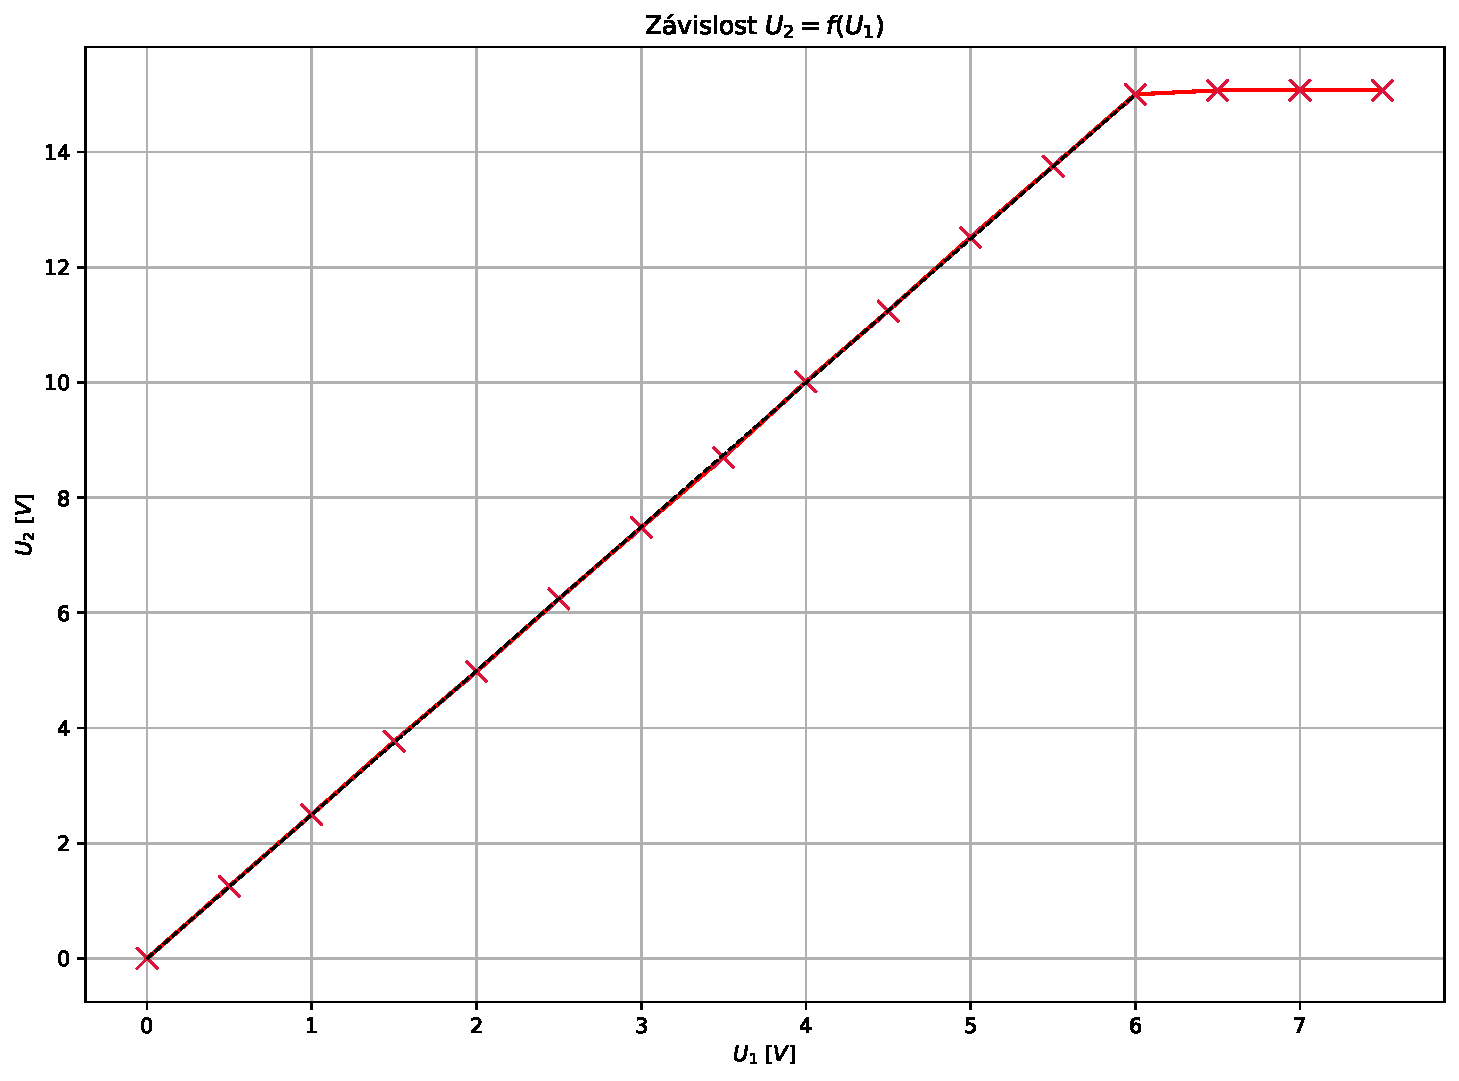
\includegraphics[width=0.9\textwidth]{grafy/graf_prevodnik_UU.pdf}
    \caption{Převodník U/U - Závislost výstupního napětí $U_2$ na vstupním napětí $U_1$}
\end{figure}

\begin{figure}[H]
    \centering
    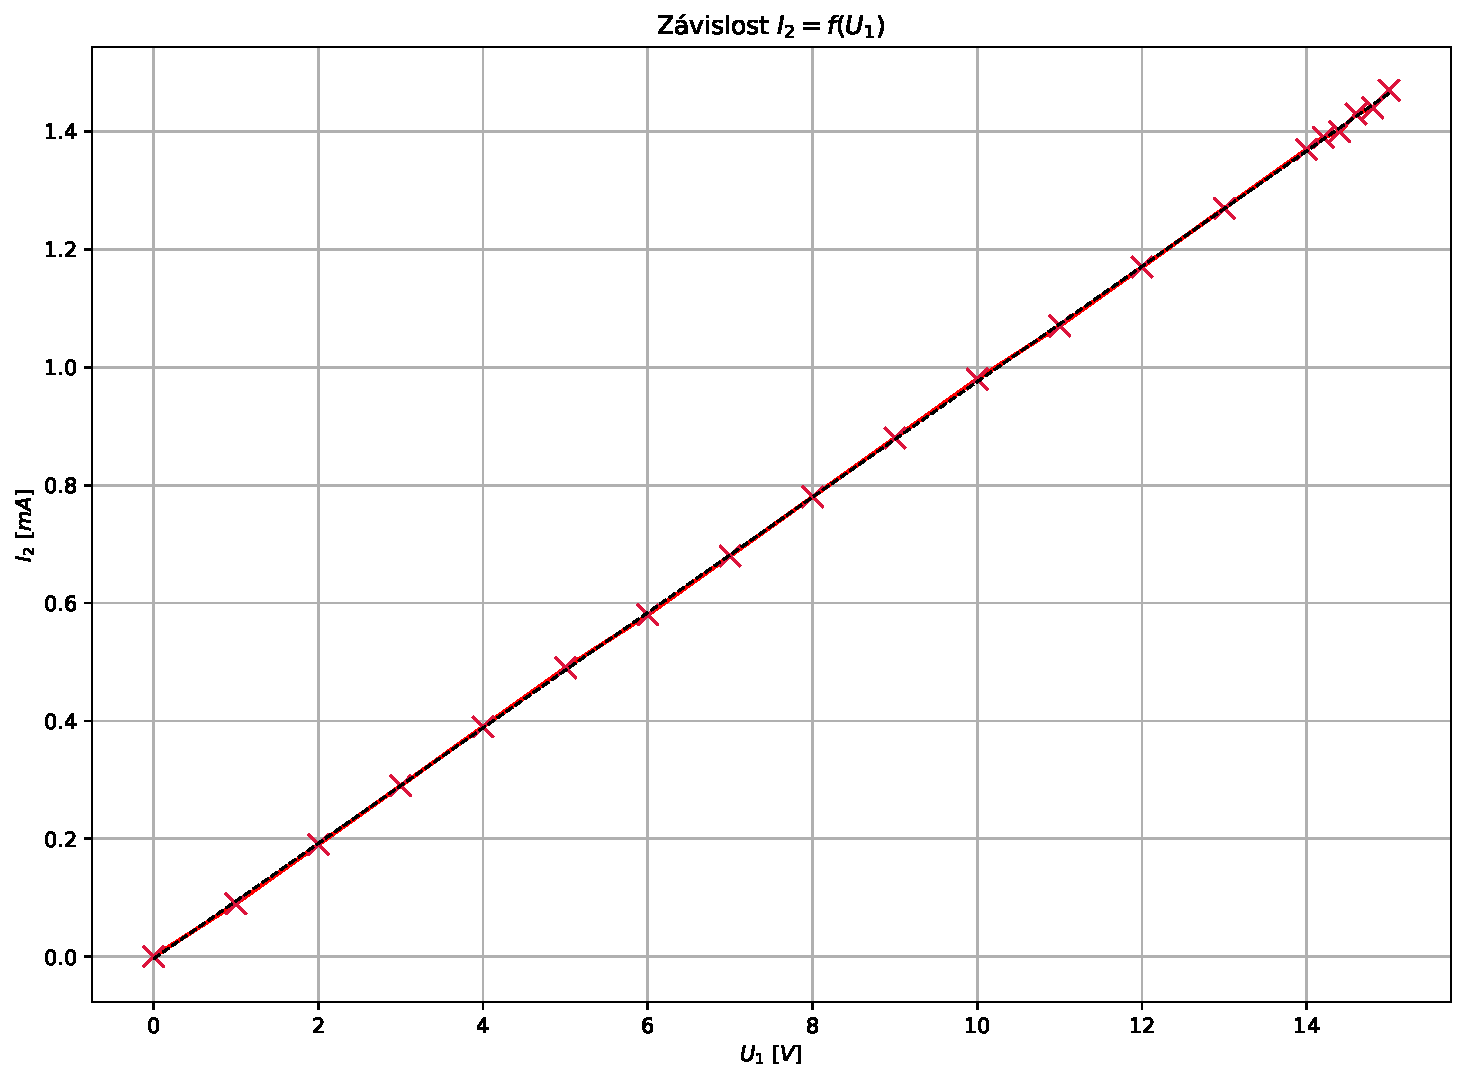
\includegraphics[width=0.9\textwidth]{grafy/graf_prevodnik_UI.pdf}
    \caption{Převodník U/I - Závislost výstupního proudu $I_2$ na vstupním napětí $U_1$}
\end{figure}

\begin{figure}[H]
    \centering
    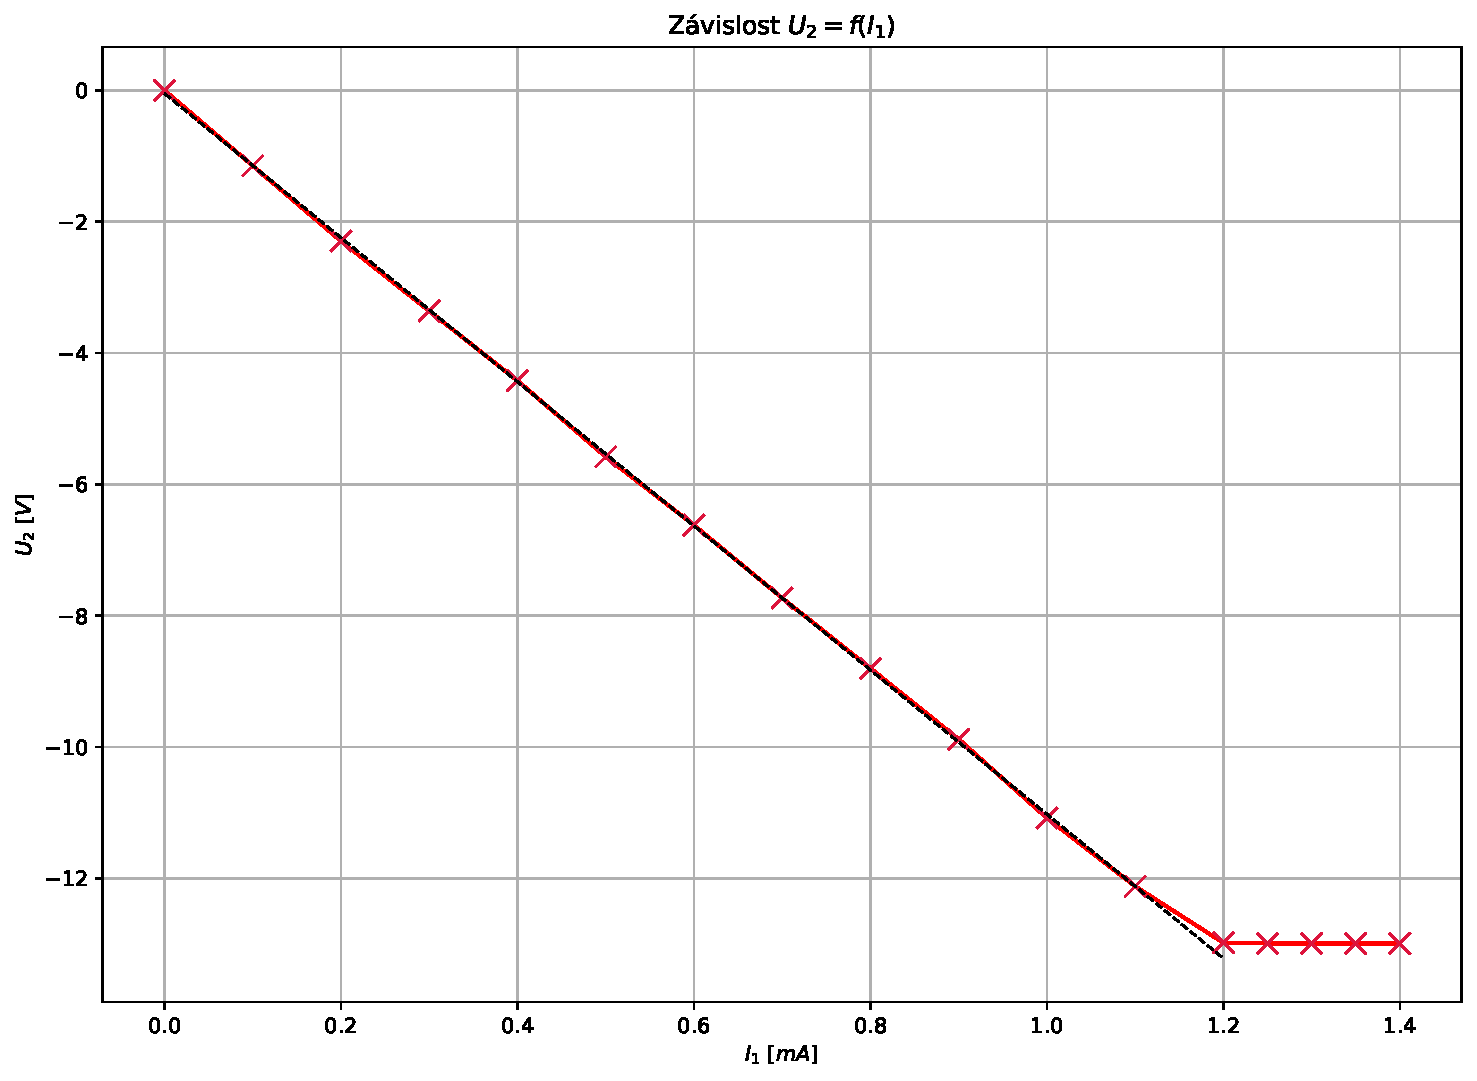
\includegraphics[width=0.9\textwidth]{grafy/graf_prevodnik_IU.pdf}
    \caption{Převodník I/U - Závislost výstupního napětí $U_2$ na vstupním proudu $I_1$}
\end{figure}

\begin{figure}[H]
    \centering
    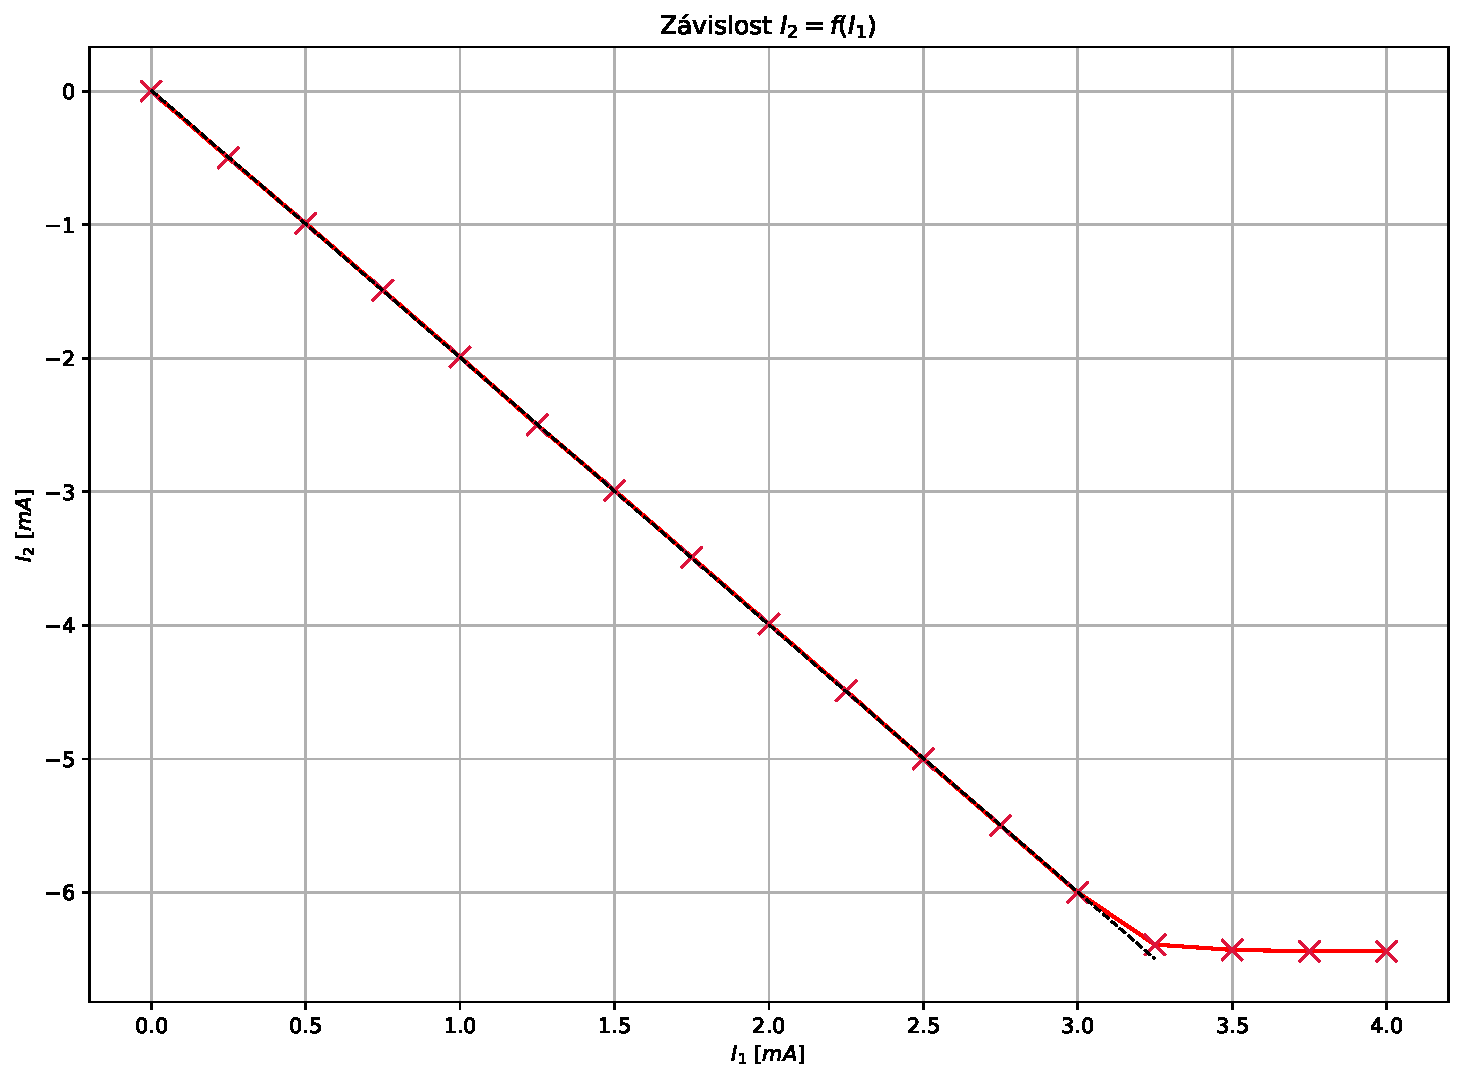
\includegraphics[width=0.9\textwidth]{grafy/graf_prevodnik_II.pdf}
    \caption{Převodník I/I - Závislost výstupního proudu $I_2$ na vstupním proudu $I_1$}
\end{figure}

\begin{figure}[H]
    \centering
    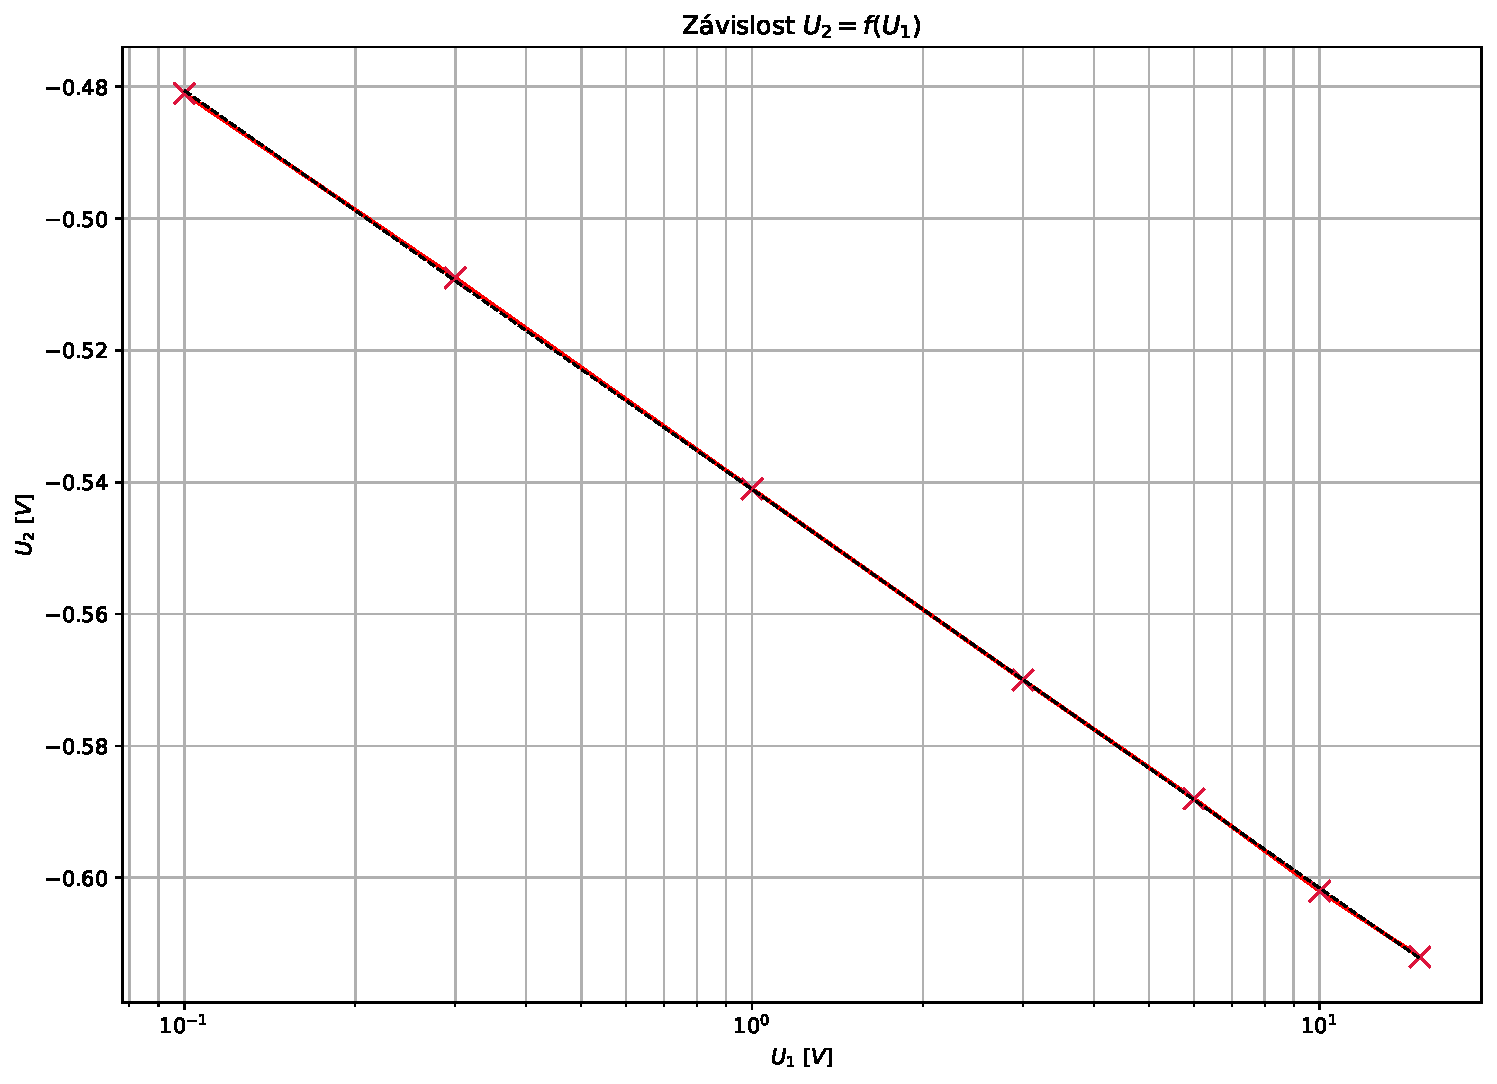
\includegraphics[width=0.9\textwidth]{grafy/graf_prevodnik_logUU.pdf}
    \caption{Převodník logU/U - Závislost výstupního napětí $U_2$ na vstupním napětí $U_1$}
\end{figure}

\subsection{Příklady výpočtu}

\begin{enumerate}
    \item Vstupní odpor převodníku
    \begin{multline*}
        R_{vst} = \textcolor{teal}{\frac{U_1}{I_1}} = \frac{1 \, V}{0,1 \cdot 10^{-6} \, A} = 10 \cdot 10^{6} \, \Omega = \underline{\underline{10 \, M \Omega}} \hfill
    \end{multline*}

    \item Převodní konstanta $A$
    \begin{multline*}
        A = \textcolor{teal}{\frac{U_2}{U_1}} = \frac{1,255 \, V}{0,5 \, V} = \underline{\underline{2,51}} \hfill
    \end{multline*}

    \item Převodní konstanta $S$
    \begin{multline*}
        S = \textcolor{teal}{\frac{I_2}{U_1}} = \frac{0,19 \cdot 10^{-3} \, A}{2 \, V} = 95 \cdot 10^{-6} \, S = \underline{\underline{95 \, \mu S}} \hfill
    \end{multline*}

    \item Převodní konstanta $W$
    \begin{multline*}
        W = \textcolor{teal}{\frac{U_2}{I_1}} = \frac{-2,295 \, V}{0,2 \cdot 10^{-3} \, A} = -11,475 \cdot 10^{3} \, \Omega = \underline{\underline{-11,48 \, k \Omega}} \hfill
    \end{multline*}

    \item Převodní konstanta $B$
    \begin{multline*}
        B = \textcolor{teal}{\frac{I_2}{I_1}} = \frac{-0,99 \cdot 10^{-3} \, A}{0,5 \cdot 10^{-3} \, A} = \underline{\underline{-1,98}} \hfill
    \end{multline*}

    \item Konstanty $K_1$ a $K_2$ - odečteno z aproximace křivky
    \begin{multline*}
        \textcolor{teal}{U_2 = K_1 \cdot log \left(U_1\right) + K_2} = -0,026 \cdot ln \left(U_1\right) - 0,5411 \hfill \\
        \ \ \ K_1 = \underline{\underline{-0,026}} \hfill \\
        \ \ \ K_2 = \underline{\underline{-0,5411}} \hfill
    \end{multline*}
\end{enumerate}

\section{Seznam použitých přístrojů}

\section{Závěr}

\end{document}